% Options for packages loaded elsewhere
\PassOptionsToPackage{unicode}{hyperref}
\PassOptionsToPackage{hyphens}{url}
%
\documentclass[
  english,
  jou]{apa7}
\usepackage{amsmath,amssymb}
\usepackage{lmodern}
\usepackage{ifxetex,ifluatex}
\ifnum 0\ifxetex 1\fi\ifluatex 1\fi=0 % if pdftex
  \usepackage[T1]{fontenc}
  \usepackage[utf8]{inputenc}
  \usepackage{textcomp} % provide euro and other symbols
\else % if luatex or xetex
  \usepackage{unicode-math}
  \defaultfontfeatures{Scale=MatchLowercase}
  \defaultfontfeatures[\rmfamily]{Ligatures=TeX,Scale=1}
\fi
% Use upquote if available, for straight quotes in verbatim environments
\IfFileExists{upquote.sty}{\usepackage{upquote}}{}
\IfFileExists{microtype.sty}{% use microtype if available
  \usepackage[]{microtype}
  \UseMicrotypeSet[protrusion]{basicmath} % disable protrusion for tt fonts
}{}
\makeatletter
\@ifundefined{KOMAClassName}{% if non-KOMA class
  \IfFileExists{parskip.sty}{%
    \usepackage{parskip}
  }{% else
    \setlength{\parindent}{0pt}
    \setlength{\parskip}{6pt plus 2pt minus 1pt}}
}{% if KOMA class
  \KOMAoptions{parskip=half}}
\makeatother
\usepackage{xcolor}
\IfFileExists{xurl.sty}{\usepackage{xurl}}{} % add URL line breaks if available
\IfFileExists{bookmark.sty}{\usepackage{bookmark}}{\usepackage{hyperref}}
\hypersetup{
  pdftitle={Increased perceptions of autonomy through choice fail to enhance motor skill retention},
  pdfauthor={Laura St.~Germain1, Allison Williams1, Noura Balbaa1, Andrew Poskus1, Olena Leshchyshen1, Keith R. Lohse2, \& Michael J. Carter1},
  pdflang={en-EN},
  pdfkeywords={Motor learning; Pre-registered; Self-controlled; Observation; Equivalence testing},
  hidelinks,
  pdfcreator={LaTeX via pandoc}}
\urlstyle{same} % disable monospaced font for URLs
\usepackage{graphicx}
\makeatletter
\def\maxwidth{\ifdim\Gin@nat@width>\linewidth\linewidth\else\Gin@nat@width\fi}
\def\maxheight{\ifdim\Gin@nat@height>\textheight\textheight\else\Gin@nat@height\fi}
\makeatother
% Scale images if necessary, so that they will not overflow the page
% margins by default, and it is still possible to overwrite the defaults
% using explicit options in \includegraphics[width, height, ...]{}
\setkeys{Gin}{width=\maxwidth,height=\maxheight,keepaspectratio}
% Set default figure placement to htbp
\makeatletter
\def\fps@figure{htbp}
\makeatother
\setlength{\emergencystretch}{3em} % prevent overfull lines
\providecommand{\tightlist}{%
  \setlength{\itemsep}{0pt}\setlength{\parskip}{0pt}}
\setcounter{secnumdepth}{-\maxdimen} % remove section numbering
% Make \paragraph and \subparagraph free-standing
\ifx\paragraph\undefined\else
  \let\oldparagraph\paragraph
  \renewcommand{\paragraph}[1]{\oldparagraph{#1}\mbox{}}
\fi
\ifx\subparagraph\undefined\else
  \let\oldsubparagraph\subparagraph
  \renewcommand{\subparagraph}[1]{\oldsubparagraph{#1}\mbox{}}
\fi
% Manuscript styling
\usepackage{upgreek}
\captionsetup{font=singlespacing,justification=justified}

% Table formatting
\usepackage{longtable}
\usepackage{lscape}
% \usepackage[counterclockwise]{rotating}   % Landscape page setup for large tables
\usepackage{multirow}		% Table styling
\usepackage{tabularx}		% Control Column width
\usepackage[flushleft]{threeparttable}	% Allows for three part tables with a specified notes section
\usepackage{threeparttablex}            % Lets threeparttable work with longtable

% Create new environments so endfloat can handle them
% \newenvironment{ltable}
%   {\begin{landscape}\begin{center}\begin{threeparttable}}
%   {\end{threeparttable}\end{center}\end{landscape}}
\newenvironment{lltable}{\begin{landscape}\begin{center}\begin{ThreePartTable}}{\end{ThreePartTable}\end{center}\end{landscape}}

% Enables adjusting longtable caption width to table width
% Solution found at http://golatex.de/longtable-mit-caption-so-breit-wie-die-tabelle-t15767.html
\makeatletter
\newcommand\LastLTentrywidth{1em}
\newlength\longtablewidth
\setlength{\longtablewidth}{1in}
\newcommand{\getlongtablewidth}{\begingroup \ifcsname LT@\roman{LT@tables}\endcsname \global\longtablewidth=0pt \renewcommand{\LT@entry}[2]{\global\advance\longtablewidth by ##2\relax\gdef\LastLTentrywidth{##2}}\@nameuse{LT@\roman{LT@tables}} \fi \endgroup}

% \setlength{\parindent}{0.5in}
% \setlength{\parskip}{0pt plus 0pt minus 0pt}

% \usepackage{etoolbox}
\makeatletter
\patchcmd{\HyOrg@maketitle}
  {\section{\normalfont\normalsize\abstractname}}
  {\section*{\normalfont\normalsize\abstractname}}
  {}{\typeout{Failed to patch abstract.}}
\patchcmd{\HyOrg@maketitle}
  {\section{\protect\normalfont{\@title}}}
  {\section*{\protect\normalfont{\@title}}}
  {}{\typeout{Failed to patch title.}}
\makeatother
\shorttitle{Autonomy-support does not benefit motor learning}
\keywords{Motor learning; Pre-registered; Self-controlled; Observation; Equivalence testing}
\usepackage{dblfloatfix}


\usepackage{csquotes}
\raggedbottom
\leftheader{\textbf{THIS PREPRINT HAS BEEN SUBMITTED FOR PEER-REVIEW}}
\rightheader{\textbf{THIS PREPRINT HAS BEEN SUBMITTED FOR PEER-REVIEW}}
\ifxetex
  % Load polyglossia as late as possible: uses bidi with RTL langages (e.g. Hebrew, Arabic)
  \usepackage{polyglossia}
  \setmainlanguage[]{english}
\else
  \usepackage[main=english]{babel}
% get rid of language-specific shorthands (see #6817):
\let\LanguageShortHands\languageshorthands
\def\languageshorthands#1{}
\fi
\ifluatex
  \usepackage{selnolig}  % disable illegal ligatures
\fi
\newlength{\cslhangindent}
\setlength{\cslhangindent}{1.5em}
\newlength{\csllabelwidth}
\setlength{\csllabelwidth}{3em}
\newenvironment{CSLReferences}[2] % #1 hanging-ident, #2 entry spacing
 {% don't indent paragraphs
  \setlength{\parindent}{0pt}
  % turn on hanging indent if param 1 is 1
  \ifodd #1 \everypar{\setlength{\hangindent}{\cslhangindent}}\ignorespaces\fi
  % set entry spacing
  \ifnum #2 > 0
  \setlength{\parskip}{#2\baselineskip}
  \fi
 }%
 {}
\usepackage{calc}
\newcommand{\CSLBlock}[1]{#1\hfill\break}
\newcommand{\CSLLeftMargin}[1]{\parbox[t]{\csllabelwidth}{#1}}
\newcommand{\CSLRightInline}[1]{\parbox[t]{\linewidth - \csllabelwidth}{#1}\break}
\newcommand{\CSLIndent}[1]{\hspace{\cslhangindent}#1}

\title{Increased perceptions of autonomy through choice fail to enhance motor skill retention}
\author{Laura St.~Germain\textsuperscript{1}, Allison Williams\textsuperscript{1}, Noura Balbaa\textsuperscript{1}, Andrew Poskus\textsuperscript{1}, Olena Leshchyshen\textsuperscript{1}, Keith R. Lohse\textsuperscript{2}, \& Michael J. Carter\textsuperscript{1}}
\date{}


\authornote{

\addORCIDlink{Laura St. Germain}{0000-0002-5513-4183}; \addORCIDlink{Keith R. Lohse}{0000-0002-7643-3887}; \addORCIDlink{Michael J. Carter}{0000-0002-0675-4271}

We have outlined author contributions using CRediT (Contributor Roles Taxonomy - \url{https://casrai.org/credit/}).

The authors made the following contributions. Laura St.~Germain: Conceptualization, Data curation, Formal analysis, Investigation - Performed the experiment, Methodology, Project administration, Software - Task Programming, Validation, Visualization, Writing - Original Draft Preparation, Writing - Review \& Editing; Allison Williams: Investigation - Performed the experiment, Writing - Original Draft Preparation, Writing - Review \& Editing; Noura Balbaa: Investigation - Performed the experiment, Writing - Original Draft Preparation, Writing - Review \& Editing; Andrew Poskus: Investigation - Performed the experiment, Writing - Review \& Editing; Olena Leshchyshen: Investigation - Performed the experiment, Writing - Review \& Editing; Keith R. Lohse: Conceptualization, Data curation, Formal analysis, Methodology, Validation, Writing - Original Draft Preparation, Writing - Review \& Editing; Michael J. Carter: Conceptualization, Data curation, Formal analysis, Funding acquisition, Methodology, Project administration, Resources, Software - Task Programming, Supervision, Validation, Visualization, Writing - Original Draft Preparation, Writing - Review \& Editing.

Correspondence concerning this article should be addressed to Michael J. Carter, 1280 Main Street West, Ivor Wynne Centre Room 203, McMaster University, Hamilton ON Canada, L8S 4K1. E-mail: \href{mailto:michaelcarter@mcmaster.ca}{\nolinkurl{michaelcarter@mcmaster.ca}}

}

\affiliation{\vspace{0.5cm}\textsuperscript{1} Department of Kinesiology, McMaster University\\\textsuperscript{2} Program in Physical Therapy, Washington University School of Medicine in Saint Louis}

\abstract{
There has been growing research interest in the effects that motivation plays in motor learning, and specifically how autonomy, competence, and social relatedness may directly benefit the learning process. Here, we present a preregistered manipulation of autonomy-support by providing learners with choice during the practice of a speed cup-stacking skill. One group was given control over when a video demonstration was provided and the viewing speed. A yoked control group received an identical demonstration schedule, but without choice (as their schedule was matched to a participant with choice). Critically, we addressed a gap in the literature by adding a yoked group who was explicitly told that they were being denied choice and that their schedule was chosen by another participant. We found no statistically significant learning differences between groups, despite finding evidence that providing choice increased perceived autonomy. Equivalence tests further showed that although the groups were not statistically equivalent, the effect size is likely too small to practically study the effects of autonomy-support through choice in most motor learning labs. These findings add to a growing body of research that questions a causal role of autonomy-support on motor learning, and the robustness of the so-called self-controlled learning advantage.
}



\begin{document}
\maketitle

A popular recommendation in recent years for creating an effective environment for motor skill learning has been to allow the learner to take control over an element of their practice that is traditionally controlled by a coach, therapist, or teacher (Sanli et al., 2013; Ste-Marie et al., 2019). This recommendation is based on the consistent finding that participants in a self-controlled (i.e., choice) group perform with higher proficiency compared to participants in a yoked (i.e., control) group on delayed retention and/or transfer tests. Participants in the yoked group do not experience the same choice opportunity provided to those in the self-controlled group. Instead, they are linked to a self-controlled participant and experience this participant's self-selected practice schedule. This so-called self-controlled learning advantage has been shown when participants are given the opportunity to schedule task difficulty (e.g., Andrieux et al., 2012; Leiker et al., 2016), the order that multiple tasks are practiced (e.g., Wu \& Magill, 2011), the frequency of watching a modeled demonstration (e.g. Wulf et al., 2005), and when to receive augmented feedback (e.g., Janelle et al., 1997; Patterson \& Carter, 2010).

Over the years, this manipulation has been described using a variety of names (e.g., self- and/or learner-controlled; -regulated; -directed; -selected), but more recently it has been subsumed by autonomy-support. In fact, autonomy-support is considered such a robust learning variable that it is one of three key pillars in the recently proposed ``OPTIMAL'' theory of motor learning (Wulf \& Lewthwaite, 2016). Wulf and Lewthwaite (2016) argued that providing learners with opportunities for choice---considered an autonomy-supportive practice manipulation---can facilitate motor performance and learning by enhancing learner's expectancies for success, and by allowing the learner to maintain their attentional focus on the task by reducing the need for self-regulatory activity (Abdollahipour et al., 2017; Chua et al., 2018; Wulf et al., 2018). In other words, these psychological and attentional benefits, and concomitant increases in performance and learning are a by-product of exercising choice during practice. Overall, autonomy-support is seen as a means to efficient goal-action coupling (Wulf \& Lewthwaite, 2016) and also links the ``OPTIMAL'' theory with Self-Determination theory (Deci \& Ryan, 2000).

Despite its prominent role within the ``OPTIMAL'' theory of motor learning, there are numerous reasons to doubt the importance of autonomy-support through the provision of choice during practice. First, if the benefits are the result of having opportunities for choice then learning differences should not emerge between different self-controlled groups. However, in experiments where different groups of participants have choice over their feedback schedule, such learning differences have been found, but not limited to, when this choice is made \emph{after} rather than before a performance attempt (Carter et al., 2014; Chiviacowsky \& Wulf, 2005), when different criteria for success are provided to participants (Chiviacowsky et al., 2012), and when the absolute number of feedback choice opportunities are limited compared to unlimited at the outset of practice (Hansen et al., 2011; Patterson et al., 2011). Second, there has been little-to-no support for the notion that practicing in a self-controlled group is perceived as more autonomy-supportive than being in a yoked group. Ste-Marie et al. (2013), for example, had participants in the self-controlled and yoked groups complete the perceived choice subscale of the Intrinsic Motivation Inventory and failed to find the expected effect of higher self-reported scores during practice in the self-controlled group. Similar findings have been reported by others (Barros et al., 2019; Carter \& Ste-Marie, 2017b; McKay \& Ste-Marie, 2020b). However, McKay and Ste-Marie (2020a) recently found that practicing in a self-controlled group was perceived as more autonomy-supportive than practicing the same task in a yoked group. This increased perceived autonomy-support did not, however, translate into enhanced learning compared to the yoked group. Although the available literature does not provide substantial evidence that self-controlled practice is autonomy-supportive, this does not necessarily mean such a manipulation is not autonomy-supportive (Altman \& Bland, 1995). For instance, this effect may in fact be quite small and require much larger sample sizes to detect than those commonly used in motor learning experiments (Lohse et al., 2016).

There are at least two other methodological issues that warrant consideration. The first of these is that in self-controlled motor learning experiments participants in the self-controlled group are usually given choice over a single component (e.g., feedback or when to watch a modeled demonstration) of their practice and participants in the yoked group are not given choice over this component. However, within the context of practice itself there are many other opportunities for choice that participants may explore, independent of their assigned group. Target-based tasks such as basketball free throws (e.g., Aiken et al., 2012) or bean-bag tossing (Grand et al., 2015) are a popular choice in motor learning experiments and have been used in self-controlled learning experiments. While a participant in the yoked group may not be permitted choice over their feedback schedule (or some other practice variable) in these experiments, this does not preclude them from opportunities for choice---and thus autonomy-support---when deciding to try different throwing techniques, speeds, and/or release points. Thus, labeling yoked groups as being devoid of choice opportunities may be a misnomer. The other consideration relates to the instructions that are provided to participants in the yoked group. In the context of feedback\footnote{While feedback is used in this example, this issue surrounding instructions is also relevant to other practice variables commonly used in self-controlled learning experiments.}, these participants are typically informed that during practice they may or may not receive feedback after a given trial (e.g., Chiviacowsky \& Wulf, 2002; Patterson \& Carter, 2010). This means that participants in yoked groups are not even aware that they have been denied an opportunity for choice, nor that their feedback schedule was created by another participant who was given choice over when feedback was or was not provided. Either of these in isolation, or both simultaneously could contribute to the consistent finding that participants in self-controlled and yoked groups report similar perceived autonomy scores when asked about their opportunities for choices with respect to the motor task (Ste-Marie et al., 2013) or about their practice environment in general (Barros et al., 2019; Carter \& Ste-Marie, 2017b; McKay \& Ste-Marie, 2020b).

\begin{table*}[tbp]

\begin{center}
\begin{threeparttable}

\caption{\label{tab:table1}Group specific instructions detailing the observation schedule that would be experienced during Acquisition.}

\begin{tabular}{ll}
\toprule
  & Acquisition instructions\\
\midrule
Self-Controlled & Before each trial, you will be asked whether you wish to watch a modeled demonstration of the task.\\
 & If you choose YES, you will then be asked whether you want to watch the video in real-time or in\\
 & slow-motion.\\
Traditional Yoked & Before each trial, you may or may not watch a modeled demonstration of the task based on a pre-\\
 & determined schedule. If you observe a model, it might be presented in real-time or in slow-motion\\
 & based on the pre-determined schedule.\\
Explicit Yoked & Before each trial, you may or may not watch a modeled demonstration of the task based on the\\
 & schedule another participant selected. If you observe a model, it might be presented in real-time or in\\
 & slow-motion based on what that participant selected.\\
\bottomrule
\end{tabular}

\end{threeparttable}
\end{center}

\end{table*}

Here we investigated the effects of making participants in a yoked group explicitly aware of not only being denied opportunities for choice over their frequency of watching and the playback speed of video demonstrations, but also that the schedule they would experience during practice was created by another participant in the experiment. The addition of this novel yoked group allowed us to address one of the previously identified methodological limitations regarding experimental group instructions in past self-controlled research. We compared the performance of this explicit yoked group with traditional self-controlled and yoked groups on a speed cup-stacking task in practice and in a delayed retention test.

\hypertarget{methods}{%
\section{Methods}\label{methods}}

We report how we determined our sample size, all data exclusions (if any), all manipulations, and all measures in the study (Simmons et al., 2012). The experimental design and analyses were preregistered using AsPredicted.org and can be viewed here: \url{https://aspredicted.org/ze8cj.pdf}.

\hypertarget{participants}{%
\subsection{Participants}\label{participants}}

One-hundred and fifty participants completed the experiment. Sample size was determined by an a priori power calculation based on our smallest comparison of interest. An early estimate for the effect of self-controlled over yoked practice was a Hedges' \(g = 0.63\) (McKay et al., 2014) and while planning this experiment this effect was estimated to be \(g = 0.52\) (Z. Yantha, personal communication, October 2019). Based on this effect, a positive correlation of \(r = 0.6\) between retention and pre-test as the covariate, and 80\% power to detect a difference between the self-controlled and traditional yoked groups, the required number of participants was 31 per group. Considering the novelty of our Explicit Yoked group, we assumed a smaller effect, \(g = 0.4\), between it and the Traditional Yoked group. With the same parameters as above, this resulted in our final sample of 50 participants per group.

Participants completed the experiment in either the Self-Controlled group \((M_{age} = 18.0\), \emph{SD} = 0.34), the Traditional Yoked group \((M_{age} = 19.5\), \emph{SD} = 1.89), or the Explicit Yoked group \((M_{age} = 19.2\), \emph{SD} = 1.55). We collected the Self-Controlled group first as their self-selected observation schedule was required for the yoking procedure for the two other groups. Once the Self-Controlled group had been collected, participants were randomly assigned to one of the two Yoked groups. All participants provided written informed consent approved by and conducted in accordance with the University's Research Ethics Board. Participants received either \$15 or a course bonus for their participation.

\hypertarget{material}{%
\subsection{Material}\label{material}}

Participants were tasked with learning the 3-6-3 speed cup stacking sequence based on the rules of the World Sport Stacking Association \href{https://www.thewssa.com/}{(https://www.thewssa.com/)}. The sequence consisted of an upstack phase and a downstack phase using official Speed Stacks cups \href{https://www.speedstacks.com/}{(https://www.speedstacks.com/)}. Participants performed the task using both their hands and had to complete an upstacking and a downstacking phase. The upstacking phase began by completing the first 3 cup pyramid, followed by the 6 cup pyramid, and then the other 3 cup pyramid. The downstacking phase began by returning to and collapsing the 3 cup pyramid that was upstacked first, then the 6 cup pyramid, and finally the last 3 cup pyramid.

\hypertarget{procedure}{%
\subsection{Procedure}\label{procedure}}

Participants completed two data collection sessions separated by approximately 24 hours. Session 1 consisted of a pre-test and an acquisition phase. Session 2 consisted of a delayed retention test. At the start of each phase of the experiment, all participants received phase-specific instructions (see Data and code availability section). Group specific instructions were provided prior to the acquisition phase (see Table \ref{tab:table1}). The instructions appeared on a 22-inch computer monitor (1920x1080 resolution) positioned to the right of the participant. Participants followed along as the instructions were read aloud by the researcher.

Each trial began with participants standing at a standard height table with their hands on marked positions on the table in front of them. The 12 cups were located in upside down stacks of 3-6-3 in front of the participant. Following a ``Get Ready!'' prompt displayed for 1 s on the monitor and a constant foreperiod of 1 s, an audiovisual ``Go-signal'' (green square and a beep tone) was presented. Participants were instructed to start stacking as quickly as possible following the ``Go-signal'' as its presentation initiated the timer. Once the upstack and downstack phases were completed, participants were instructed to press the spacebar on a keyboard located in front of them to stop the timer. If an error occurred (e.g., only completed the upstack phase then stopped the timer, forgot to hit the timer, etc), the experimenter recorded the trial number for later removal.

The pre-test and delayed retention test both consisted of five no-feedback trials. The acquisition phase had 25 trials and was the only phase where the video demonstration could be watched based on group assignment. Participants in the Self-Controlled group could decide at the start of each trial if they wanted to watch the video demonstration. If they chose to watch the video, they were then asked whether they wanted to watch it in real-time or slow motion (35\% of real-time). The real-time video was 6 s in duration and the slow motion version was 18 s. To ensure a constant viewing period of 18 s, a blank screen was shown for 12 s following the end of the real-time video. If they chose not to watch the video, a blank screen was shown for 18 s. Participants in the Traditional Yoked and Explicit Yoked groups received the demonstration schedule created by a participant in the Self-Controlled group with the exception that participants in the Explicit Yoked group were made aware that this schedule was created by another participant. Feedback about stacking time (s) was displayed for 2 s after every acquisition trial.

To test predictions based on the ``OPTIMAL'' theory regarding the role of motivation, enhanced expectancies, and autonomy-support, participants completed the interest/enjoyment and perceived competence subscales from the Intrinsic Motivation Inventory (McAuley et al., 1989) and a custom scale regarding choice used in previous self-controlled motor learning experiments (Barros et al., 2019; Carter \& Ste-Marie, 2017b). The order of questions from each scale were randomized and each question was rated using a 7-point Likert scale. Participants answered these questions after the pre-test, after trials five and 25 of acquisition, and before the delayed retention test.

A custom LabVIEW (National Instruments Inc.) program was created that controlled the presentation of all instructions, the video demonstrations, the timing of the experimental protocol, and recorded and stored the data for later analysis.

\hypertarget{data-analysis}{%
\subsection{Data analysis}\label{data-analysis}}

Our primary outcome measure was stacking time (i.e., response time) in seconds. Trials recorded as errors \((76/5250 = 1.45\%)\) during data collection were manually removed prior to data analysis. For each participant, pre-test and delayed retention trials were aggregated into one block of five trials and acquisition was aggregated into five blocks of five trials. Significance level was set to 0.05 for all statistical tests. Effect sizes for omnibus tests are reported using generalized eta squared \((\eta^2_{G})\) or eta squared \((\eta^2)\). Post hoc comparisons were conducted using Holm's correction. A Cook's distance of \(\geq 1\) was used to identify any influential cases.

\hypertarget{results}{%
\section{Results}\label{results}}

\hypertarget{pre-registered-analysis}{%
\subsection{Pre-registered analysis}\label{pre-registered-analysis}}

To test whether delayed retention (Figure \ref{fig:fig1}C) was differentially impacted by the experimental group (i.e., Self-Controlled, Traditional Yoked, Explicit Yoked) experienced during acquisition, we performed a one-way ANCOVA controlling for pre-test. As can be seen, the Self-Controlled group \((M = 9.99\), \(95\%CI = [9.68,10.31])\), the Traditional Yoked group \((M = 10.18\), \(95\%CI = [9.86,10.50])\), and the Explicit Yoked group \((M = 10.12\), \(95\%CI = [9.81,10.44])\) all had similar stacking times in retention (means are shown as the adjusted means controlling for pre-test). The effect of Group was not significant, \(F(2,146) = .335\), \(p = .716\), \(\eta^2 = .002\).



\begin{figure*}

{\centering 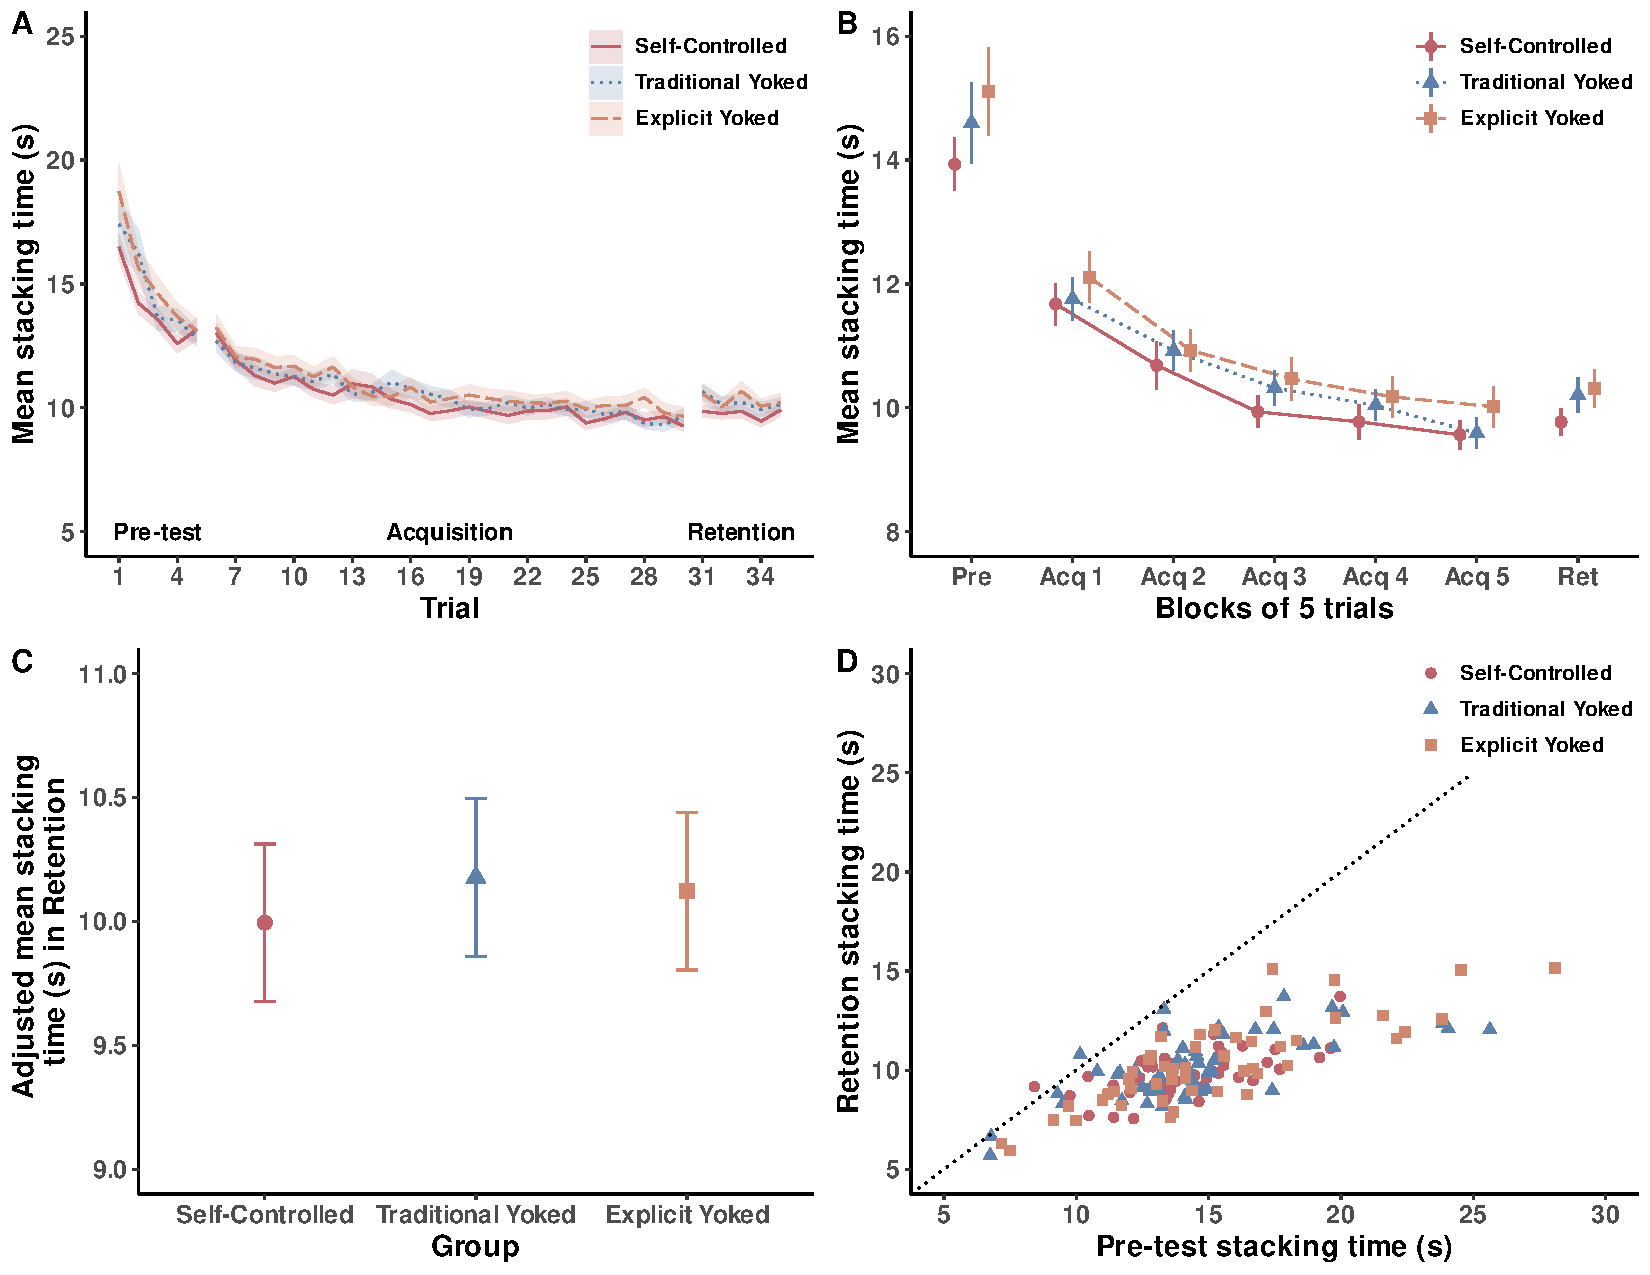
\includegraphics[width=1\linewidth,height=1\textheight]{../../figs/fig1} 

}

\caption{Physical performance data of the experiment. The Self-Controlled group is shown in red with solid lines and/or circles, the Traditional Yoked group is shown in blue with dotted and/or triangles, and the Explicit Yoked group is shown in orange with dashed and/or squares. \textbf{A}. Trial-by-trial stacking time (s) data averaged across participants within each group (shaded area represents standard error). Splits between line segments denote the end of one phase and the start of the next. Pre-test (Trials 1 to 5) and Acquisition (Trials 6 to 30) occurred on Day 1 and Retention (Trials 31 to 35) occurred on Day 2, approximately 24-hours later. \textbf{B}. Mean stacking time (s) for each group was computed by averaging the data from \textbf{A} into 7 blocks of trials. Error bars represent 95\% confidence intervals. Splits between line segments denote the end of one phase and the start of the next. \textbf{C}. Mean stacking time (s) adjusted for pre-test for each group. Error bars represent 95\% confidence intervals. \textbf{D}. Scatterplot showing the relationship between each participant's mean stacking time (s) in pre-test and retention.}\label{fig:fig1}
\end{figure*}

\begin{table*}[t]

\begin{center}
\begin{threeparttable}

\caption{\label{tab:table2}The mean frequencies for each acquisition block of requesting to watch the video demonstration and choosing the regular viewing speed.}

\begin{tabular}{llllll}
\toprule
  & Block 1 & Block 2 & Block 3 & Block 4 & Block 5\\
\midrule
Model viewing frequency & 32.6\% & 16.9\% & 12.0\% & 12.9\% & 9.3\%\\
 &  &  &  &  & \\
Regular speed frequency & 33.8\% & 38.1\% & 50.0\% & 34.4\% & 30.4\%\\
\bottomrule
\end{tabular}

\end{threeparttable}
\end{center}

\end{table*}

\hypertarget{non-pre-registered-analyses}{%
\subsection{Non pre-registered analyses}\label{non-pre-registered-analyses}}

\hypertarget{traditional-self-controlled-learning-advantage}{%
\subsubsection{Traditional self-controlled learning advantage}\label{traditional-self-controlled-learning-advantage}}

To investigate whether a traditional self-controlled learning advantage existed---that is a comparison between the Self-Controlled and Traditional Yoked groups---we analyzed the non-adjusted retention scores using a Welch's \emph{t}-test. The analysis revealed that the Self-Controlled group \((M = 9.77\), \(95\%CI = [9.55,9.99])\) and the Traditional Yoked group \((M = 10.20\), \(95\%CI = [9.92,10.49])\) were not statistically different, \(t(88.10) = 1.45\), \(p = .15\), \(g = .29\).

\hypertarget{acquisition-phase}{%
\subsubsection{Acquisition phase}\label{acquisition-phase}}

Model frequency and the video speed request data are reported in Table \ref{tab:table2}. The mean frequency of viewing the video demonstration during acquisition was \(16.7\%\). When a video demonstration was selected, the mean frequency that the regular speed was selected was \(37.3\%\). Stacking time for each Group decreased across acquisition trials (Figure \ref{fig:fig1}A) and blocks (Figure \ref{fig:fig1}B). A 3 Group x 5 Block mixed ANOVA with repeated measures on Block revealed a significant Block effect, \(F(3.63,533.79) = 116.73\), \(p < .001\), \(\eta^2_{G} = .133\). Post hoc comparisons revealed all acquisition blocks were significantly different from each other. Both the Group effect, \(F(2,147) = .738\), \(p = .48\), \(\eta^2_{G} = .008\), and Group x Block interaction, \(F(7.26,533.79) = .543\), \(p = .802\), \(\eta^2_{G} = .001\), were not statistically significant.

\hypertarget{perceived-autonomy}{%
\subsubsection{Perceived autonomy}\label{perceived-autonomy}}

Self-reported perceived autonomy scores are displayed in Figure \ref{fig:fig2}A where it can be seen that the Self-Controlled group reported slightly higher scores compared to the two Yoked groups at all time points following the pre-test. A 3 Group x 3 Time ANCOVA controlling for pre-test revealed a significant Group effect, \(F(2,146) = 8.04\), \(p < .001\), \(\eta^2_{G} = .083.\) Post hoc comparisons on the adjusted means revealed that the Self-Controlled group \((M = 5.61\), \(95\%CI =[5.42,5.80])\) had significantly higher perceptions of autonomy compared to both the Traditional Yoked group \((M = 5.13\), \(95\%CI = [4.94,5.32])\) and the Explicit Yoked group \((M = 5.13\), \(95\%CI = [4.94,5.32])\), which did not differ from each other (and were, in fact, identical to two decimal places). Both the Time effect, \(F(1.61,234.98) = .867\), \(p = .400\), \(\eta^2_{G} = .001\), and Group x Time interaction, \(F(3.22,234.98) = 2.10\), \(p = .096\), \(\eta^2_{G} = .005\), were not significant.



\hypertarget{intrinsic-motivation}{%
\subsubsection{Intrinsic motivation}\label{intrinsic-motivation}}

Self-reported intrinsic motivation scores can be found in Figure \ref{fig:fig2}B. At each time point, all groups reported similar scores on the interest/enjoyment subscale. A 3 Group x 3 Time ANCOVA controlling for pre-test revealed non-significant effects for Group, \(F(2,146) = 2.08\), \(p = .129\), \(\eta^2_{G} = .024\), Time, \(F(1.68,245.73) = .563\), \(p = .541\), \(\eta^2_{G} = .001\), and the Group x Time interaction, \(F(3.37,245.73) = .333\), \(p = .824\), \(\eta^2_{G} = .001\).

\hypertarget{perceived-competence}{%
\subsubsection{Perceived competence}\label{perceived-competence}}

The scores from the perceived competence subscale at each time point are displayed in Figure \ref{fig:fig2}C. As can be seen, perceived competence scores showed a modest increase over time followed by a slight decrease before the delayed retention test. A 3 Group x 3 Time ANCOVA controlling for pre-test showed an effect of Time, \(F(1.75,255.22) = 10.60\), \(p < .001\), \(\eta^2_{G} = .015\). Post hoc tests on adjusted means revealed that scores were rated as significantly higher at the end of acquisition \((M = 3.98\), \(95\%CI = [3.67,3.89])\) and before retention \((M = 3.78\), \(95\%CI = [3.67,3.89])\) compared to after trial 5 \((M = 3.60\), \(95\%CI = [3.49,3.71])\). However, perceived competence was significantly lower before retention compared to the end of acquisition. No significant effect of Group, \(F(2,146) = 2.65\), \(p = .074\), \(\eta^2_{G} = .028\), or Group x Time interaction, \(F(3.50,255.22) = .549\), \(p = .677\), \(\eta^2_{G} = .002\), was found.

\hypertarget{equivalence-tests}{%
\subsubsection{Equivalence tests}\label{equivalence-tests}}

To further probe our null effects (Harms \& Lakens, 2018) related to our main predictions, two equivalence tests (Self-Controlled versus Traditional Yoked and Traditional Yoked versus Explicit Yoked) on pre-test adjusted retention stacking times were carried out using the two one-sided test procedure (Lakens et al., 2018; Schuirmann, 1987). To establish our smallest effect size of interest (Lakens, 2021) we calculated the effect size our design had 33\% power to detect (Simonsohn, 2015), which was \(d_{s} = .31\). The Self-Controlled and Traditional Yoked groups were not statistically different, \(t(97.99) = -0.830\), \(p = 0.409\), and not statistically equivalent, \(t(97.99) = 0.720\), \(p = 0.237\), given equivalence bounds of \(-.355\) and \(.355\) (on a raw scale). Similarly, the Traditional Yoked and Explicit Yoked groups were not statistically different, \(t(97.99) = 0.262\), \(p = 0.794\), and not statistically equivalent, \(t(97.99) = -1.288\), \(p = 0.100\), given equivalence bounds of \(-.355\) and \(.355\) (on a raw scale).

\begin{figure*}

{\centering 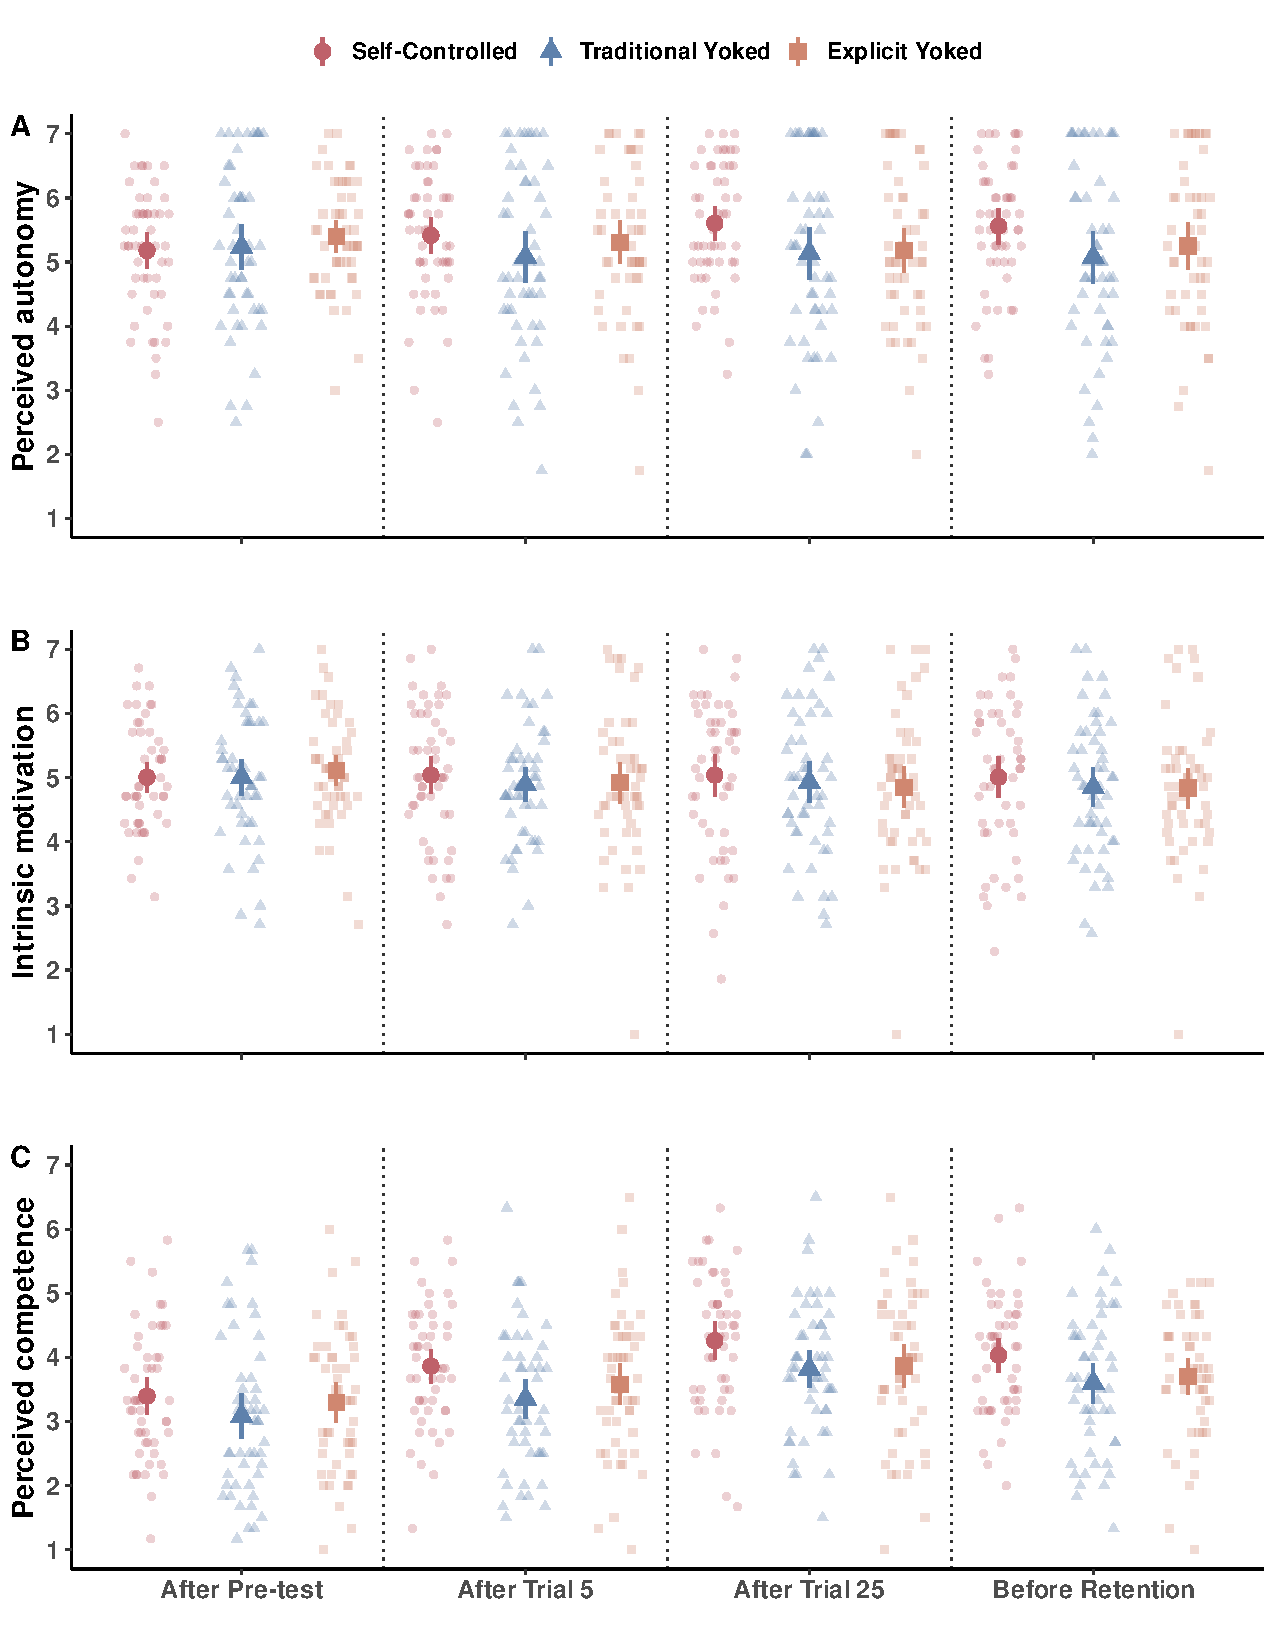
\includegraphics[width=0.85\linewidth,height=0.85\textheight]{../../figs/fig2} 

}

\caption{Questionnaire data. Groups means for \textbf{A} perceived autonomy, \textbf{B} intrinsic motivation, and \textbf{C} perceived competence after pre-test, trial 5, and trial 25 on Day 1, and before retention on Day 2. The Self-Controlled group is shown in red circles, the Traditional Yoked group is shown in blue triangles, and the Explicit Yoked group is shown in orange squares. Dots represent individual participants in each group. Scores could range from 1 (Strongly disagree) to 7 (Strongly agree). Error bars represent 95\% confidence intervals.}\label{fig:fig2}
\end{figure*}

\hypertarget{discussion}{%
\section{Discussion}\label{discussion}}

It has been argued that self-controlled practice conditions are effective for motor learning because they are autonomy-supportive in nature (Wulf \& Lewthwaite, 2016). Yet, this claim has received, at best, modest support in the motor learning literature (e.g., McKay \& Ste-Marie, 2020a; but see Barros et al., 2019; Carter \& Ste-Marie, 2017b; Ste-Marie et al., 2013 for non-support). Here, we addressed a possible methodological limitation for this lack of support. That is, in previous self-controlled motor learning research, participants in the yoked group are not made aware that they have been denied opportunities to exercise choice over a practice variable such as feedback or watching a modeled demonstration. In the present experiment we introduced a novel yoked group that was explicitly told that the observation schedule---frequency and speed of video---they would receive during practice was actually one created by another participant in the experiment. Contrary to our prediction, the Explicit Yoked group did not report significantly lower perceived autonomy scores than the Traditional Yoked group, which was only informed their observation schedule was predetermined. In line with the ``OPTIMAL'' theory (Wulf \& Lewthwaite, 2016), the Self-Controlled group reported significantly higher perceived autonomy-support than both the Traditional and Explicit Yoked groups. However, this boost in perceived autonomy did not lead to enhanced motor performance or learning. These findings from a well-powered experiment are difficult to reconcile with a core pillar of the ``OPTIMAL'' theory of motor learning.

\hypertarget{self-controlled-practice-conditions-as-autonomy-supportive}{%
\subsection{Self-controlled practice conditions as autonomy-supportive}\label{self-controlled-practice-conditions-as-autonomy-supportive}}

A common problem with many of the self-controlled or choice motor learning literature claiming autonomy-support as an underlying mechanism for self-controlled learning advantages is a failure to include measures that actually test this claim (e.g., Chiviacowsky, 2014; Chiviacowsky et al., 2012; Lewthwaite et al., 2015). Instead, this link to autonomy-support is merely assumed based on the provision of choice to one group of participants versus not giving the same choice to another group of participants. As noted earlier, an issue with this assumption is that within the practice environment itself, there are myriad opportunities for participants, independent of group, to exercise choice. In throwing tasks common to motor learning, participants can explore the task workspace by attempting different throwing techniques. In more lab-based tasks that consist of multiple spatial and timing goals (e.g., waveform matching), participants can choose a single goal to focus on and master before shifting their attention to another goal. Commensurate with this idea, Ste-Marie et al. (2013) found no differences in perceived choice regarding the motor task being learned between their self-controlled and yoked groups, despite the self-controlled group showing enhanced retention. This may explain why research has consistently reported perceived autonomy scores that do not differ significantly between self-controlled and yoked groups (Barros et al., 2019; Carter \& Ste-Marie, 2017b; McKay \& Ste-Marie, 2020b).

Another possible explanation for the finding that being in a self-controlled group has not been perceived as more autonomy-supportive than being in a yoked group is that choice is typically provided over a single element of the practice variable, such as the frequency of receiving feedback (e.g., Aiken et al., 2012; Carter \& Ste-Marie, 2017a) or the level of task difficulty (Andrieux et al., 2012; Leiker et al., 2016). Control or choice over a single dimension may not be strong enough to elicit a large enough boost in perceived autonomy above and beyond that of being able to explore one's task workspace as mentioned above. Thus, to increase the saliency of the self-controlled manipulation in the present experiment, we gave the self-controlled participants control over two elements of their observation schedule: viewing frequency and video playback speed. Having control of these two dimensions resulted in higher perceptions of autonomy in our Self-Controlled group compared to the Traditional and Explicit Yoked groups. This may explain the inconsistency with past research failing to find this effect (Barros et al., 2019; Carter \& Ste-Marie, 2017b; McKay \& Ste-Marie, 2020b; Ste-Marie et al., 2013). However, McKay and Ste-Marie (2020a) recently found that choice over a single element increased perceived autonomy, but similar to our data they also did not find this led to increased learning. Thus, it is unclear whether the higher autonomy scores in the present experiment can in fact be attributed to having control over multiple elements of one's observation schedule.

In a similar vein, past research has also suggested that self-controlled learning benefits are not dependent on the amount of choice opportunities over a single element (Patterson et al., 2011). Given these findings, we argue that the most likely explanation for the inconsistency surrounding the effect of self-controlled practice being autonomy-supportive is that this effect is quite small, and the designs of previous experiments have lacked the statistical power to reliability detect this effect. These experiments have had sample sizes of 20 participants or less per group, whereas there were 50 participants in each group in the present experiment and 64 per group (when collapsed across constant and variable practice schedules) in McKay and Ste-Marie (2020a). Collapsing across our two yoked groups, we estimate an effect of autonomy-support of \(g = .197\) whereas the estimate from McKay and Ste-Marie (2020a) was \(g = .57\). Regardless of the estimated size of the effect for autonomy-support through a self-controlled practice condition, a larger issue and challenge to the ``OPTIMAL'' theory is that significantly higher perceptions of autonomy did not result in superior performance in either acquisition or delayed retention (Wulf \& Lewthwaite, 2016).

\hypertarget{no-learning-advantage-from-a-self-controlled-observation-schedule}{%
\subsection{No learning advantage from a self-controlled observation schedule}\label{no-learning-advantage-from-a-self-controlled-observation-schedule}}

The delayed retention results in the present experiment not only are inconsistent with numerous past experiments reporting a self-controlled motor learning benefit (for a review see Ste-Marie et al., 2019), but also the general consensus that the self-controlled learning advantage is a robust effect (Wulf \& Lewthwaite, 2016). Of late, however, there has been an increase in the number of papers reporting a failure to detect the so-called self-controlled learning advantage (e.g., Barros et al., 2019; Grand et al., 2017; McKay \& Ste-Marie, 2020a, 2020b). This recent lack of support may arise from the self-controlled learning advantage being a much smaller effect than originally estimated (\(g = 0.63\) by McKay et al.~2014). A more recent estimate of this effect from a meta-analysis using a weight-function model was \(g = .11, \,95\% CI = [.047, .18]\) (McKay et al., 2021). This estimate was further reduced to \(g = .054\) after controlling for publication bias using the precision-effect estimate with standard error (PEESE) method. Thus, both models seem to suggest a trivial effect for self-controlled learning. Additional simulations included in the meta-analysis provided plausible effect size estimates ranging from \(g = -.11\) to \(.26\) (i.e., it could even favour being in the yoked group). In our experiment, the estimated effect size of self-controlled versus yoked (collapsed across our Traditional and Explicit Yoked groups) was \(g = 0.22\). While this estimate is larger than those from the weight-function model and PEESE method, it does fall within the range of plausible effect sizes (McKay et al., 2021). When the lack of a self-controlled advantage in previous work and our current experiment are contextualized within the findings of this recent meta-analysis, it is not as surprising that the so-called self-controlled learning benefit was not replicated.

Despite the large sample size of the present experiment (\emph{n}/group = 50) versus the typical self-controlled motor learning experiment (median \emph{n}/group = 18 based on the experiments included in the meta-analysis by McKay et al.~2021), the results of the primary analysis and the equivalence tests remain inconclusive. This, along with the effect size estimates in the recent meta-analysis, suggest enormous sample sizes are required to reliably detect an effect of a self-controlled learning advantage. Using the upper bound, \(g = .26\), of the range of plausible effects, \emph{253 participants} are required to have 80\% power to detect this effect in retention using an independent-samples \emph{t}-test. The number of participants jumps to \emph{1300 per group}, if for instance the estimate from the weight-function model, \(g = .11\), is accurate (McKay et al., 2021). Given the field of motor learning suffers from a lack of adequately powered designs (Lohse et al., 2016) and that underpowered designs are more likely to produce false positives and overestimated effect sizes (Button et al., 2013), we are skeptical of the replicability of the previous overwhelming support for the self-controlled learning advantage.

\hypertarget{lack-of-support-for-key-predictions-of-the-optimal-theory-of-motor-learning}{%
\subsection{Lack of support for key predictions of the ``OPTIMAL'' theory of motor learning}\label{lack-of-support-for-key-predictions-of-the-optimal-theory-of-motor-learning}}

Within the ``OPTIMAL'' theory (Wulf \& Lewthwaite, 2016), it is predicted that practice conditions that promote autonomy-support and enhance expectancies contribute to a virtuous cycle that leads to superior motor performance and learning. In other words, significant group differences between self-controlled and yoked groups would be expected on measures related to these psychological constructs. As mentioned earlier, we found higher perceptions of autonomy-support in our Self-Controlled group relative to the Traditional and Explicit Yoked groups; however, this did not enhance motor learning as predicted within the virtuous cycle. Contrary to the ``OPTIMAL'' theory, we did not find an effect of group for perceived competence (i.e., enhanced expectancies) or intrinsic motivation. Perceived competence scores did increase across acquisition blocks, which mirrors the improved motor performance seen throughout acquisition. These results are in line with results of a path analysis that suggested self-efficacy (i.e., enhanced expectancies) and intrinsic motivation were insufficient to explain self-controlled learning benefits (Ste-Marie et al., 2016). Overall, our results are inconsistent with key predictions of the ``OPTIMAL'' theory regarding autonomy-support and enhanced expectancies, and further question the causal role such manipulations play in motor learning.

In sum, we found that being able to control two aspects of one's observation schedule during practice was perceived as autonomy-supportive relative to not having this same control opportunity. However, making participants in an Explicit Yoked group aware they would be denied a control opportunity during practice did not decrease perceptions of autonomy relative to participants in the Traditional Yoked group. Furthermore, we did not find evidence than an autonomy-supportive manipulation had any direct causal effect on learning and we also failed to replicate the typical self-controlled learning advantage. It is worth noting that in some situations autonomy-support in and of itself might be a desired affective outcome (Ste-Marie et al., 2020). In such circumstance, providing learners with choice opportunities may be a useful motivationally-protective outcome. However, such a tool should be used judiciously as it is typically motor outcomes in the form of relatively permanent performance changes that is the true goal of any motor learning intervention (Ste-Marie et al., 2020). Ultimately, our results add to a growing body of evidence that questions whether autonomy-supportive manipulations directly affect learning. One explanation for this lack of replicability is that the \emph{``true''} effect of such manipulations are much smaller than previously estimated (McKay et al., 2021). Given the resources required (in terms of sample size) to reliably detect the tiny effects, we encourage motor learning scientists to invest their limited resources carefully---either studying practice conditions that have much bigger effects or devising ways to reduce variability and increase power through clever experimental design (McClelland, 2000).

\hypertarget{conflict-of-interest}{%
\section{Conflict of interest}\label{conflict-of-interest}}

The authors declare no competing interests.

\hypertarget{funding}{%
\section{Funding}\label{funding}}

This work was supported by the Natural Sciences and Engineering Research Council (NSERC) of Canada (RGPIN-2018-05589; MJC). LSG was also supported by an NSERC PGS-D scholarship.

\hypertarget{data-and-code-availability}{%
\section{Data and code availability}\label{data-and-code-availability}}

All material, data, and scripts to reproduce our analyses and figures can be accessed here: \url{https://github.com/cartermaclab/expt_explicit-yoked}.

\hypertarget{r-packages-used-in-this-project}{%
\section{R packages used in this project}\label{r-packages-used-in-this-project}}

R {[}Version 4.0.5; R Core Team (2021){]} and the R-packages \emph{cowplot} {[}Version 1.1.1; Wilke (2020){]}, \emph{jmv} {[}Version 1.2.23; Selker et al. (2020){]}, \emph{papaja} {[}Version 0.1.0.9997; Aust and Barth (2020){]}, \emph{pwr} {[}Version 1.3.0; Champely (2020){]}, \emph{tidyverse} {[}Version 1.3.1; Wickham et al. (2019){]}, and \emph{TOSTER} {[}Version 0.3.4; Lakens (2017){]}.

\newpage

\hypertarget{references}{%
\section{References}\label{references}}

\begingroup
\interlinepenalty = 10000
\setlength{\parindent}{-0.5in}
\setlength{\leftskip}{0.5in}

\endgroup

\hypertarget{refs}{}
\begin{CSLReferences}{1}{0}
\leavevmode\hypertarget{ref-abdollahipour2017}{}%
Abdollahipour, R., Palomo Nieto, M., Psotta, R., \& Wulf, G. (2017). External focus of attention and autonomy support have additive benefits for motor performance in children. \emph{Psychology of Sport and Exercise}, \emph{32}, 17--24. \url{https://doi.org/10.1016/j.psychsport.2017.05.004}

\leavevmode\hypertarget{ref-aiken2012}{}%
Aiken, C. A., Fairbrother, J. T., \& Post, P. G. (2012). The effects of self-controlled video feedback on the learning of the basketball set shot. \emph{Frontiers in Psychology}, \emph{3}. \url{https://doi.org/10.3389/fpsyg.2012.00338}

\leavevmode\hypertarget{ref-altman1995}{}%
Altman, D. G., \& Bland, J. M. (1995). Statistics notes: Absence of evidence is not evidence of absence. \emph{BMJ}, \emph{311}(7003), 485. \url{https://doi.org/10.1136/bmj.311.7003.485}

\leavevmode\hypertarget{ref-andrieux2012}{}%
Andrieux, M., Danna, J., \& Thon, B. (2012). Self-control of task difficulty during training enhances motor learning of a complex coincidence-anticipation task. \emph{Research Quarterly for Exercise and Sport}, \emph{83}(1), 27--35. \url{https://doi.org/10.1080/02701367.2012.10599822}

\leavevmode\hypertarget{ref-R-papaja}{}%
Aust, F., \& Barth, M. (2020). \emph{{papaja}: {Create} {APA} manuscripts with {R Markdown}}. \url{https://github.com/crsh/papaja}

\leavevmode\hypertarget{ref-barros2019}{}%
Barros, J. A. C., Yantha, Z. D., Carter, M. J., Hussien, J., \& Ste-Marie, D. M. (2019). Examining the impact of error estimation on the effects of self-controlled feedback. \emph{Human Movement Science}, \emph{63}, 182--198. \url{https://doi.org/10.1016/j.humov.2018.12.002}

\leavevmode\hypertarget{ref-button2013}{}%
Button, K. S., Ioannidis, J. P. A., Mokrysz, C., Nosek, B. A., Flint, J., Robinson, E. S. J., \& Munafò, M. R. (2013). Power failure: why small sample size undermines the reliability of neuroscience. \emph{Nature Reviews Neuroscience}, \emph{14}(5), 365--376. \url{https://doi.org/10.1038/nrn3475}

\leavevmode\hypertarget{ref-carter2014}{}%
Carter, M. J., Carlsen, A. N., \& Ste-Marie, D. M. (2014). Self-controlled feedback is effective if it is based on the learner{'}s performance: A replication and extension of chiviacowsky and wulf (2005). \emph{Frontiers in Psychology}, \emph{5}. \url{https://doi.org/10.3389/fpsyg.2014.01325}

\leavevmode\hypertarget{ref-carter2017b}{}%
Carter, M. J., \& Ste-Marie, D. M. (2017a). An interpolated activity during the knowledge-of-results delay interval eliminates the learning advantages of self-controlled feedback schedules. \emph{Psychological Research}, \emph{81}(2), 399--406. \url{https://doi.org/10.1007/s00426-016-0757-2}

\leavevmode\hypertarget{ref-carter2017a}{}%
Carter, M. J., \& Ste-Marie, D. M. (2017b). Not all choices are created equal: Task-relevant choices enhance motor learning compared to task-irrelevant choices. \emph{Psychonomic Bulletin \& Review}, \emph{24}(6), 1879--1888. \url{https://doi.org/10.3758/s13423-017-1250-7}

\leavevmode\hypertarget{ref-R-pwr}{}%
Champely, S. (2020). \emph{Pwr: Basic functions for power analysis}. \url{https://CRAN.R-project.org/package=pwr}

\leavevmode\hypertarget{ref-chiviacowsky2014}{}%
Chiviacowsky, S. (2014). Self-controlled practice: Autonomy protects perceptions of competence and enhances motor learning. \emph{Psychology of Sport and Exercise}, \emph{15}(5), 505--510. \url{https://doi.org/10.1016/j.psychsport.2014.05.003}

\leavevmode\hypertarget{ref-chiviacowsky2005}{}%
Chiviacowsky, S., \& Wulf, G. (2005). Self-controlled feedback is effective if it is based on the learner's performance. \emph{Research Quarterly for Exercise and Sport}, \emph{76}(1), 42--48. \url{https://doi.org/10.1080/02701367.2005.10599260}

\leavevmode\hypertarget{ref-chiviacowsky2002}{}%
Chiviacowsky, S., \& Wulf, G. (2002). Self-controlled feedback: Does it enhance learning because performers get feedback when they need it? \emph{Research Quarterly for Exercise and Sport}, \emph{73}(4), 408--415. \url{https://doi.org/10.1080/02701367.2002.10609040}

\leavevmode\hypertarget{ref-chiviacowsky2012}{}%
Chiviacowsky, S., Wulf, G., \& Lewthwaite, R. (2012). Self-controlled learning: The importance of protecting perceptions of competence. \emph{Frontiers in Psychology}, \emph{3}. \url{https://doi.org/10.3389/fpsyg.2012.00458}

\leavevmode\hypertarget{ref-chua2018}{}%
Chua, L.-K., Wulf, G., \& Lewthwaite, R. (2018). Onward and upward: Optimizing motor performance. \emph{Human Movement Science}, \emph{60}, 107--114. \url{https://doi.org/10.1016/j.humov.2018.05.006}

\leavevmode\hypertarget{ref-deci2000}{}%
Deci, E. L., \& Ryan, R. M. (2000). The {"}what{"} and {"}why{"} of goal pursuits: Human needs and the self-determination of behavior. \emph{Psychological Inquiry}, \emph{11}(4), 227--268. \url{https://doi.org/10.1207/S15327965PLI1104_01}

\leavevmode\hypertarget{ref-grand2015}{}%
Grand, K. F., Bruzi, A. T., Dyke, F. B., Godwin, M. M., Leiker, A. M., Thompson, A. G., Buchanan, T. L., \& Miller, M. W. (2015). Why self-controlled feedback enhances motor learning: Answers from electroencephalography and indices of motivation. \emph{Human Movement Science}, \emph{43}, 23--32. \url{https://doi.org/10.1016/j.humov.2015.06.013}

\leavevmode\hypertarget{ref-grand2017}{}%
Grand, K. F., Daou, M., Lohse, K. R., \& Miller, M. W. (2017). Investigating the Mechanisms Underlying the Effects of an Incidental Choice on Motor Learning. \emph{Journal of Motor Learning and Development}, \emph{5}(2), 207--226. \url{https://doi.org/10.1123/jmld.2016-0041}

\leavevmode\hypertarget{ref-hansen2011}{}%
Hansen, S., Pfeiffer, J., \& Patterson, J. T. (2011). Self-control of feedback during motor learning: Accounting for the absolute amount of feedback using a yoked group with self-control over feedback. \emph{Journal of Motor Behavior}, \emph{43}(2), 113--119. \url{https://doi.org/10.1080/00222895.2010.548421}

\leavevmode\hypertarget{ref-harms2018}{}%
Harms, C., \& Lakens, D. (2018). Making 'null effects' informative: Statistical techniques and inferential frameworks. \emph{Journal of Clinical and Translational Research}. \url{https://doi.org/10.18053/jctres.03.2017S2.007}

\leavevmode\hypertarget{ref-janelle1997}{}%
Janelle, C. M., Barba, D. A., Frehlich, S. G., Tennant, L. K., \& Cauraugh, J. H. (1997). Maximizing performance feedback effectiveness through videotape replay and a self-controlled learning environment. \emph{Research Quarterly for Exercise and Sport}, \emph{68}(4), 269--279. \url{https://doi.org/10.1080/02701367.1997.10608008}

\leavevmode\hypertarget{ref-lakens2021}{}%
Lakens, D. (2021). \emph{Sample size justification}. \url{https://doi.org/10.31234/osf.io/9d3yf}

\leavevmode\hypertarget{ref-R-TOSTER}{}%
Lakens, D. (2017). Equivalence tests: A practical primer for t-tests, correlations, and meta-analyses. \emph{Social Psychological and Personality Science}, \emph{1}, 1--8. \url{https://doi.org/10.1177/1948550617697177}

\leavevmode\hypertarget{ref-lakens2018}{}%
Lakens, D., Scheel, A. M., \& Isager, P. M. (2018). Equivalence Testing for Psychological Research: A Tutorial. \emph{Advances in Methods and Practices in Psychological Science}, \emph{1}(2), 259--269. \url{https://doi.org/10.1177/2515245918770963}

\leavevmode\hypertarget{ref-leiker2016}{}%
Leiker, A. M., Bruzi, A. T., Miller, M. W., Nelson, M., Wegman, R., \& Lohse, K. R. (2016). The effects of autonomous difficulty selection on engagement, motivation, and learning in a motion-controlled video game task. \emph{Human Movement Science}, \emph{49}, 326--335. \url{https://doi.org/10.1016/j.humov.2016.08.005}

\leavevmode\hypertarget{ref-lewthwaite2015}{}%
Lewthwaite, R., Chiviacowsky, S., Drews, R., \& Wulf, G. (2015). Choose to move: The motivational impact of autonomy support on motor learning. \emph{Psychonomic Bulletin \& Review}, \emph{22}(5), 1383--1388. \url{https://doi.org/10.3758/s13423-015-0814-7}

\leavevmode\hypertarget{ref-lohse2016}{}%
Lohse, K., Buchanan, T., \& Miller, M. (2016). Underpowered and Overworked: Problems With Data Analysis in Motor Learning Studies. \emph{Journal of Motor Learning and Development}, \emph{4}(1), 37--58. \url{https://doi.org/10.1123/jmld.2015-0010}

\leavevmode\hypertarget{ref-mcauley1989}{}%
McAuley, E., Duncan, T., \& Tammen, V. V. (1989). Psychometric properties of the intrinsic motivation inventory in a competitive sport setting: A confirmatory factor analysis. \emph{Research Quarterly for Exercise and Sport}, \emph{60}(1), 48--58. \url{https://doi.org/10.1080/02701367.1989.10607413}

\leavevmode\hypertarget{ref-mcclelland2000}{}%
McClelland, G. H. (2000). Increasing statistical power without increasing sample size. \emph{American Psychologist}, \emph{55}(8), 963--964. https://doi.org/\url{https://psycnet.apa.org/doi/10.1037/0003-066X.55.8.963}

\leavevmode\hypertarget{ref-mckay2014}{}%
McKay, B., Carter, M. J., \& Ste-Marie, D. M. (2014). Self-controlledlearning: A meta-analysis. \emph{Journal of Sport \& Exercise Psychology,} \emph{36}, S43.

\leavevmode\hypertarget{ref-mckay2020a}{}%
McKay, B., \& Ste-Marie, D. M. (2020a). Autonomy support via instructionally irrelevant choice not beneficial for motor performance or learning. \emph{Research Quarterly for Exercise and Sport}, \emph{0}(0), 1--13. \url{https://doi.org/10.1080/02701367.2020.1795056}

\leavevmode\hypertarget{ref-mckay2020b}{}%
McKay, B., \& Ste-Marie, D. M. (2020b). Autonomy support and reduced feedback frequency have trivial effects on learning and performance of a golf putting task. \emph{Human Movement Science}, \emph{71}(1026124). \url{https://doi.org/10.1016/j.humov.2020.102612}

\leavevmode\hypertarget{ref-mckay2021}{}%
McKay, B., Yantha, Z. D., Hussien, J., Carter, M. J., \& Ste-Marie, D. M. (2021). \emph{Meta-analytic findings in the self-controlled motor learning literature: Underpowered, biased, and lacking evidential value}. \url{https://doi.org/10.31234/osf.io/8d3nb}

\leavevmode\hypertarget{ref-patterson2010}{}%
Patterson, J. T., \& Carter, M. (2010). Learner regulated knowledge of results during the acquisition of multiple timing goals. \emph{Human Movement Science}, \emph{29}(2), 214--227. \url{https://doi.org/10.1016/j.humov.2009.12.003}

\leavevmode\hypertarget{ref-patterson2011}{}%
Patterson, J. T., Carter, M., \& Sanli, E. (2011). Decreasing the proportion of self-control trials during the acquisition period does not compromise the learning advantages in a self-controlled context. \emph{Research Quarterly for Exercise and Sport}, \emph{82}(4), 624--633. \url{https://doi.org/10.1080/02701367.2011.10599799}

\leavevmode\hypertarget{ref-R-base}{}%
R Core Team. (2021). \emph{R: A language and environment for statistical computing}. R Foundation for Statistical Computing. \url{https://www.R-project.org/}

\leavevmode\hypertarget{ref-sanli2013}{}%
Sanli, E. A., Patterson, J. T., Bray, S. R., \& Lee, T. D. (2013). Understanding self-controlled motor learning protocols through the self-determination theory. \emph{Frontiers in Psychology}, \emph{3}. \url{https://doi.org/10.3389/fpsyg.2012.00611}

\leavevmode\hypertarget{ref-schuirmann1987}{}%
Schuirmann, D. J. (1987). A comparison of the Two One-Sided Tests Procedure and the Power Approach for assessing the equivalence of average bioavailability. \emph{Journal of Pharmacokinetics and Biopharmaceutics}, \emph{15}(6), 657--680. \url{https://doi.org/10.1007/BF01068419}

\leavevmode\hypertarget{ref-R-jmv}{}%
Selker, R., Love, J., \& Dropmann, D. (2020). \emph{Jmv: The 'jamovi' analyses}. \url{https://CRAN.R-project.org/package=jmv}

\leavevmode\hypertarget{ref-simmons2012}{}%
Simmons, J. P., Nelson, L. D., \& Simonsohn, U. (2012). \emph{A 21 Word Solution}. \url{https://doi.org/10.2139/ssrn.2160588}

\leavevmode\hypertarget{ref-simonsohn2015}{}%
Simonsohn, U. (2015). Small Telescopes: Detectability and the Evaluation of Replication Results. \emph{Psychological Science}, \emph{26}(5), 559--569. \url{https://doi.org/10.1177/0956797614567341}

\leavevmode\hypertarget{ref-ste-marie2016}{}%
Ste-Marie, D. M., Carter, M. J., Law, B., Vertes, K., \& Smith, V. (2016). Self-controlled learning benefits: Exploring contributions of self-efficacy and intrinsic motivation via path analysis. \emph{Journal of Sports Sciences}, \emph{34}(17), 1650--1656. \url{https://doi.org/10.1080/02640414.2015.1130236}

\leavevmode\hypertarget{ref-ste-marie2019}{}%
Ste-Marie, D. M., Carter, M. J., \& Yantha, Z. D. (2019). \emph{Self-controlled learning: Current findings, theoretical perspectives, and future directions} (3rd ed.). Routledge.

\leavevmode\hypertarget{ref-ste-marie2020}{}%
Ste-Marie, D. M., Lelievre, N., \& Germain, L. S. (2020). Revisiting the applied model for the use of observation: A review of articles spanning 2011{{}}2018. \emph{Research Quarterly for Exercise and Sport}, \emph{91}(4), 594--617. \url{https://doi.org/10.1080/02701367.2019.1693489}

\leavevmode\hypertarget{ref-ste-marie2013}{}%
Ste-Marie, D. M., Vertes, K. A., Law, B., \& Rymal, A. M. (2013). Learner-controlled self-observation is advantageous for motor skill acquisition. \emph{Frontiers in Psychology}, \emph{3}. \url{https://doi.org/10.3389/fpsyg.2012.00556}

\leavevmode\hypertarget{ref-R-tidyverse}{}%
Wickham, H., Averick, M., Bryan, J., Chang, W., McGowan, L. D., François, R., Grolemund, G., Hayes, A., Henry, L., Hester, J., Kuhn, M., Pedersen, T. L., Miller, E., Bache, S. M., Müller, K., Ooms, J., Robinson, D., Seidel, D. P., Spinu, V., \ldots{} Yutani, H. (2019). Welcome to the {tidyverse}. \emph{Journal of Open Source Software}, \emph{4}(43), 1686. \url{https://doi.org/10.21105/joss.01686}

\leavevmode\hypertarget{ref-R-cowplot}{}%
Wilke, C. O. (2020). \emph{Cowplot: Streamlined plot theme and plot annotations for 'ggplot2'}. \url{https://CRAN.R-project.org/package=cowplot}

\leavevmode\hypertarget{ref-wu2011}{}%
Wu, W. F. W., \& Magill, R. A. (2011). Allowing learners to choose. \emph{Research Quarterly for Exercise and Sport}, \emph{82}(3), 449--457. \url{https://doi.org/10.1080/02701367.2011.10599777}

\leavevmode\hypertarget{ref-wulf2016}{}%
Wulf, G., \& Lewthwaite, R. (2016). Optimizing performance through intrinsic motivation and attention for learning: The OPTIMAL theory of motor learning. \emph{Psychonomic Bulletin \& Review}, \emph{23}(5), 1382--1414. \url{https://doi.org/10.3758/s13423-015-0999-9}

\leavevmode\hypertarget{ref-wulf2018}{}%
Wulf, G., Lewthwaite, R., Cardozo, P., \& Chiviacowsky, S. (2018). Triple play: Additive contributions of enhanced expectancies, autonomy support, and external attentional focus to motor learning. \emph{Quarterly Journal of Experimental Psychology}, \emph{71}(4), 824--831. \url{https://doi.org/10.1080/17470218.2016.1276204}

\leavevmode\hypertarget{ref-wulf2005}{}%
Wulf, G., Raupach, M., \& Pfeiffer, F. (2005). Self-controlled observational practice enhances learning. \emph{Research Quarterly for Exercise and Sport}, \emph{76}(1), 107--111. \url{https://doi.org/10.1080/02701367.2005.10599266}

\end{CSLReferences}


\end{document}
